\documentclass [bachelor,german,a4paper,11pt,oneside,webreferences,glossary,acronym,listofabbrev,indextop,nolistoftables,nolistoflistings,nolistofalgorithms]{INSOthesis}
% change encoding in the document
\inputencoding{utf8} % default
%\inputencoding{latin1} % for windows

\thesistitle{Evaluierung von REST Frameworks für Android}
\thesisshorttitle{Evaluierung von REST Frameworks}
\thesissubtitle{im Kontext des Revex2020 Projekts} % optional
\thesisdate{\today}

% all titles and designations have to be gender-related!
%\thesistype{Diplomarbeit}{Master's Thesis}
%\thesisdegree{Diplom-Ingenieurin}{Diplom-Ingenieurin}
\thesiscurriculum{Software \& Information Engineering}{Software \& Information Engineering} % your study
\thesisauthor{Elisabeth Pilz} % your name
\thesisauthoraddress{Luegstraße 13, 3340 Waidhofen Ybbs} % your address
\thesismatrikelno{1225231} % your registration number

% advisor
%\thesisauthorpreamble {Verfasser}
%\thesisadvisorpreamble {Betreuung}
%\thesisadvisorone {Thomas Grechenig}
\thesisadvisortwo {Dominik Moser}
%\thesisadvisorthree {Vorname Nachname}

% Bibliographie file
\bibliography{bibliography/references}

\hypersetup{
  %colorlinks=false % enable and disable frames arround links
}

%%%%%%%%%%%%%%%%%%%%%%%%%%%%%%%%%%%%%%%%%%%%%
%
% Can be used to add additional informations
%
%%%%%%%%%%%%%%%%%%%%%%%%%%%%%%%%%%%%%%%%%%%%%
% \AfterTitlePages{}
% \AfterDeclaration{}
% \AfterAcknowledgements{}
% \AfterAbstract{}
% \AfterListOfFigures{}
% \AfterListOfTables{}
% \AfterAbbreviations{}
% \AfterBibliography{}
\renewcommand\afterchapternum{\hspace{1em}}
\begin{document}

\maketitle

%%%%%%%%%%%%%%%%%%%%%%%%%%%%%%%%%%%%%%%%%
%%%   CONTENTS    %%%%%%%%%%%%%%%%%%%%%%%
%%%%%%%%%%%%%%%%%%%%%%%%%%%%%%%%%%%%%%%%%

%%%%%%%%%%%%%%%%%%%%%%%%%%%%%%%%%%%%%%%%%%%%%%%%%%%%%%%%%%%%%%%%%%%%%%%%
\chapter{Einleitung}
\label{sec:introduction}
%%%%%%%%%%%%%%%%%%%%%%%%%%%%%%%%%%%%%%%%%%%%%%%%%%%%%%%%%%%%%%%%%%%%%%%%

%=======================================================================
\section{Problemstellung}
%=======================================================================
Einer der größten Trends auf den Business-Markt ist die Mobilisierung der Geschäftswelt, die sich in den verschiedensten Unternehmensstrategien widerspiegelt. Es gibt zahlreiche Innovationen, um unabhängig von Stakeholdern, Zeit, Ort und Geräten auf Daten und Anwendungen zuzugreifen. Ein wesentlicher Innovationsstrang ist dabei die Entwicklung von Business-Apps, um beispielsweise die Arbeitszeiten auf Geschäftsreisen effektiv ausnützen zu können. Dadurch hat die Bedeutung der Informations- und Kommunikationsindustrie in den letzten Jahren in den Unternehmen stetig zugenommen \cite{smartMobileApps1}.
\\\\
Durch die immer stärkere Nachfrage nach mobilen Apps im Arbeitsalltag ist es notwendig, mobile Endgräte in bestehende Geschäftsprozesse der Unternehmen zu integrieren. Dabei soll es vermieden werden, eine komplett neue IT-Infrastruktur unter Beteiligung von mobilen Endgeräten zu schaffen. In vielen Unternehmen wird daher die IT-Anwendungslandschaft an das Paradigma der serviceorientierten Architektur ausgerichtet. Ein wesentlicher Vorteil dabei ist, dass wohl definierte Schnittstellen vorhanden sind und angebotene Dienste flexibel und plattformunabhängig genutzt werden können. Sollen nur mobile Anwendungen in die existierende IT-Anwendungslandschaft eingegliedert werden, bedeutet dies in der serviceorientierten Architektur, das Web Services benötigt werden. In der Praxis werden Web Services entweder mit dem Kommunikationsprotokoll \acrfull{SOAP} oder \acrfull{REST} umgesetzt \cite{smartMobileApps17}.
\\\\
Im Revex2020 Projekt wird das Kommunikationsprotokoll REST verwendet, dadurch ist es nötig ein geeignetes Framework aufseiten der mobilen App zu finden, dass eine vollständige und korrekte Anbindung an den Webservice ermöglicht. Es existieren bereits zahlreiche Frameworks, die eine REST Implementierung unterstützen, diese unterscheiden sich aber stark in der Qualität und im Funktionsumfang. Auch bieten nicht alle diese Frameworks eine Unterstützung für Android an. Daher ist die Auswahl eines geeigneten Frameworks für eine erfolgreiche Implementierung ausschlaggebend. 

%=======================================================================
\section{Motivation}
%=======================================================================

Die Thematik rund um REST-Frameworks für Android ist noch relativ neu, dadurch ist es nicht möglich ohne größere Recherchen ein geeignetes Framework für das Projekt Revex2020 auszuwählen. Es gibt zwar einige Vergleiche von REST Frameworks, wie etwa die Fachstudie von Markus Fischer, Kalman Kepes und Alexander Wassiljew \cite{vergleich13}. In dieser Studie wird allerdings nicht darauf eingegangen, ob die Frameworks eine Implementierung clientseitig mit Android unterstützen, es wird die vermehrt auf die serverseitige Implementierung eingegangen. Die Möglichkeit der clientseitigen Implementierung ist aber eine essenzielle Anforderung, da eine Business-App für Android entwickelt werden soll. 
\\\\
Der immer stärker wachsende Bereich von mobilen Anwendungen macht das zu untersuchende Thema besonders interessant. Herkömmliche Software rückt immer weiter in den Hintergrund, Daten sollen sofort und überall abgerufen werden können. Mobile Endgeräte wie Smartphone und Tablets verändern daher die Geschäftswelt nachhaltig, Führungskräfte und Mitarbeiter erhalten jederzeit Zugang zu Unternehmensinformationen und -prozessen. Die Unternehmen der Zukunft werden daher mobil \cite{smartMobileApps7}.  
\\\\
Revex2020 ist ein Forschungsprojekt zur Revitalisierung von Wasserkraftwerken, das in Kooperation mit dem Institut für Energietechnik und Thermodynamik entwickelt wird \cite{doujak}. Ein Ziel dieses Projektes ist es, Mitarbeitern zukünftig zu ermöglichen, mithilfe von mobilen Endgeräten den Zustand einzelner Kraftwerkskomponenten vor Ort erfassen zu können. Es soll eine Android-App entwickelt werden, die das bereits vorhandene Backend, über das REST-Webservices nutzt um exemplarisch den Anwendungsfall abzubilden.

%=======================================================================
\section{Zielsetzung}
%=======================================================================

Ziel dieser Bachelorarbeit ist die Evaluierung verschiedener REST-Frameworks für Android im Kontext des Revex2020 Projekts, um eine unkomplizierte Anbindung an das bereits vorhandene Backend zu ermöglichen. Dazu werden bestehende REST-Frameworks für Android getestet, indem diese in einem Anwendungsfall eingesetzt werden. Nach der Evaluierung dieser Frameworks soll eine Empfehlung abgegeben werden, welches sich am besten für das Revex2020 Projekt eignet.
\\\\
Die Evaluierung der Frameworks erfolgt anhand von Prototypen, indem die REST-Frameworks verwendet werden. Es wurden im Vorfeld verschiedene Anwendungsfälle definiert (siehe Abbildung \ref{figure:useCase}), indem die einzelnen REST Frameworks integriert werden. Dabei werden in einem Szenario verschiedene Prozesse durchgespielt, wie Kraftwerk erstellen, löschen, bearbeiten und anzeigen. Als Vorlage dazu wurde die bestehende Web-Applikation des Projektes verwendet.
\\\\

\begin{minipage}{\textwidth} 
	\centering	
	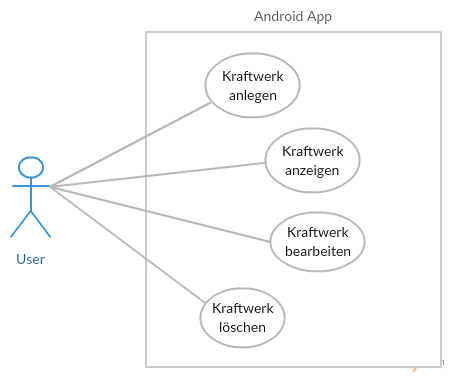
\includegraphics[width=0.65\textwidth]{figures/kraftwerke_use_case.png}
	\captionof{figure}{Use-Case-Diagramm}
	\label{figure:useCase}
	\vspace{2ex}
\end{minipage}

%=======================================================================
\section{Methodik}
\label{sec:methodik}
%=======================================================================
Die Qualität der einzelnen Frameworks soll anhand folgender Kriterien verglichen werden, welche an dem Kriterienkatalog der Fachstudie "Vergleich von Frameworks zur Implementierung von REST-basierten Anwendungen" \cite{vergleich13} angelehnt sind. Dieser Kriterienkatalog beschäftigt sich mit den Eigenschaften für die Evaluierung von REST Frameworks, vor allem auf serverseitiger Sicht. Der Kriterienkatalog wurde deshalb gekürzt bzw. einzelne Punkte zusammengefasst und abgeändert, um eine Evaluierung im Kontext des Projektes Revex2020 durchführen zu können. 
\\\\
Das Hauptaugenmerk der Evaluierung liegt auf der Clientseite, da die entwickelte App eine Client Applikation darstellt. Deswegen wurden spezifische Kriterien der Fachstudie zu einer REST Server Applikation gestrichen. Beispielsweise wurde der gesamte Kriterienblock über Ressourcentypen \cite{ressourcen:rest} weggelassen, da es für die clientseitige Verarbeitung irrelevant ist, welche Ressourcentypen serverseitig implementiert werden können. 
\\\\
\textbf{Entwicklungskultur rund um die Frameworks:}
\begin{itemize}
	\item Unter welcher Lizenz steht das Projekt zur Verfügung?
	\item Existiert eine aktive Community?
	\item Ist eine Dokumentation des Codes vorhanden? (Schnittstellenbeschreibung, JavaDoc)	
	\item Gibt es Hilfestellung für Entwicklung? (Tutorial, Codebeispiele)
\end{itemize}

\textbf{Implementierung der REST-Frameworks:}
\begin{itemize}
	\item Wie aufwendig ist es das Framework ins Projekt einzubinden? 
	\item Welche HTTP-Methoden werden unterstützt? (GET, POST, PUT, DELETE etc.)
	\item Gibt es Möglichkeiten den HTTP-Header zu verändern oder zu erweitern?
	\item Welche Medientypen werden unterstützt? (JSON, HTML, XML etc.)
	\item Kann die URL zum Abfragen von Resourcen dynamisch verändert werden? (z.B. über Parameter steuern)
	\item Gibt es eine Möglichkeit für asynchronen Nachrichtenaustausch?
	\item Wird das HATEOAS-Konzept* unterstützt?
	\item Wird ein Error-Handling unterstützt?	
\end{itemize}

\textbf{Performance und benötige Speicherplatz der Frameworks:}
\begin{itemize}
	\item Wie stark wird die CPU belastet?  
	\item Wie viel RAM wird benötigt? 
	\item Wie schnell erfolgt die Abwicklung einzelner Requests (GET, POST)?
	\item Wie groß ist die erzeugte .apk-Datei?	
\end{itemize}
\newpage
\textbf{Erweiterte Technische Fähigkeiten der Frameworks:}
\begin{itemize}
	\item Wie wird Sicherheit gehandhabt?  (Authentifizierung)
	\item Werden andere Protokolle fernab von HTTP unterstützt?	
	\item Unterstützt das Framework die Entwicklung von Server Applikationen?
	\item Bietet das Framework zusätzliche Dienst fernab der REST-Kommunikation an?
	\item Wird transaktionales Verhalten vom Framework unterstützt? (ACID**-Eigenschaften)\\
\end{itemize}

* Das \textbf{HATEOAS}-Konzept wird in Kapitel \ref{sec:rest} genauer beschrieben.
\\\\
** \textbf{ACID} seht für Atomicity, Consistency, Isolation und Durability. Dieses Konzept beschreibt, dass alle Daten die während einer Transaktion verwendet werden, gesperrt sind und sich nicht ändern dürfen, so lange bis die Transaktion Commited wird oder ein Rollback durchgeführt wird. Das Einhalten dieser Eigenschaften ist wichtig, da die Kommunikation zu Servern über zustandslose REST-Schnittstellen abgewickelt wird. Durch die Zustandslosigkeit der Anfragen kann es bei Fehlern schnell zu einer Dateninkonsistenz auf dem Server kommen \cite{braun:Transaktionen}.

%%%%%%%%%%%%%%%%%%%%%%%%%%%%%%%%%%%%%%%%%%%%%%%%%%%%%%%%%%%%%%%%%%%%%%%%
\chapter{State of the Art}
\label{sec:stateOfTheArt}
%%%%%%%%%%%%%%%%%%%%%%%%%%%%%%%%%%%%%%%%%%%%%%%%%%%%%%%%%%%%%%%%%%%%%%%%

Um Rest Frameworks für die Evaluierung zu finden, wurde eine Technologierecherche durchgeführt. Dabei konnten folgende Projekte gefunden werden, welche eine REST-Anbindung für Android unterstützen:
\begin{itemize}
	\item Resty (\href{http://beders.github.io/Resty/Resty/Overview.html}{http://beders.github.io/Resty/Resty/Overview.html})
	\item Retrofit (\href{http://square.github.io/retrofit/}{http://square.github.io/retrofit/})
	\item RESTlet (\href{http://restlet.com/}{http://restlet.com/})
	\item Spring for Android (\href{http://projects.spring.io/spring-android/}{http://projects.spring.io/spring-android/})
	\item CRest (\href{http://crest.codegist.org/index.html}{http://crest.codegist.org/index.html})
	\item RESTeasy Mobile (\href{http://resteasy.jboss.org/}{http://resteasy.jboss.org/})
	\item RESTDroid (\href{http://pcreations.fr/me/restdroid-resource-oriented-rest-client-for-android}{http://pcreations.fr/me/restdroid-resource-oriented-rest-client-for-android})
	\item Jersey (\href{https://jersey.java.net/}{https://jersey.java.net/})
\end{itemize}

Es würde den Rahmen der Bachelorarbeit überschreiten, all diese gefundenen REST Frameworks zu evaluieren. Es wurde daher einer Vorstudie gemacht, aufgrund derer die Drei populärsten und den Anforderungen adäquatesten Frameworks ausgewählt wurden.
\\\\
Die Popularität eines Frameworks gibt eine gewisse Auskunft über die Qualität, da für diese Frameworks oft besserer Support in Form von Dokumentation zur Verfügung steht. Eine Studie von Chris Parnin\cite{parnin2012crowd} beschäftigen sich damit, wie "'Crowd documentation"' beispielsweise auf Question and Answer (Q\&A) Webseiten, die Hilfestellung zu verschiedenen Frameworks beeinflusst. Verwenden viele Entwickler ein Framework, sind dadurch mehr Fragen auf Q\&A Webseiten vorhanden und dadurch können mögliche Fragen besser beantwortet werden. Durch eine Erhebung der Anzahl von Fragen auf Stack Overflow\footnote{\href{http://stackoverflow.com/}{http://stackoverflow.com/}} und der Stars auf GitHub\footnote{\href{https://github.com/}{https://github.com/}} wurden Rückschlüsse auf die Popularität der einzelnen Frameworks gezogen.  
\\\\
In dem Artikel "'How to identify a strong open source project"\cite{balter:strongOS} werden verschiedene Indikatoren erhoben, welche Rückschlüsse auf eine solide und gute Entwicklung eines Frameworks geben. Deswegen wurden zusätzlich noch verschiedene Aktivitäten auf GitHub verglichen, wie Datum des letzten Commits oder Anzahl der Commits.

\begin{minipage}{\textwidth} 
	\centering	
	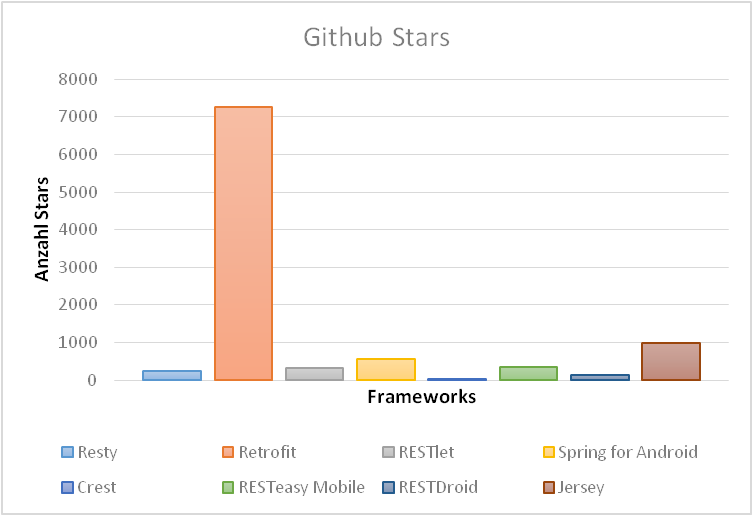
\includegraphics[width=0.65\textwidth]{figures/github_stars.png}
	\captionof{figure}{Github Stars, abgerufen am 25.09.2015}
	\label{figure:githubStars}
	\vspace{2ex}
\end{minipage}

\begin{minipage}{\textwidth} 
	\centering	
	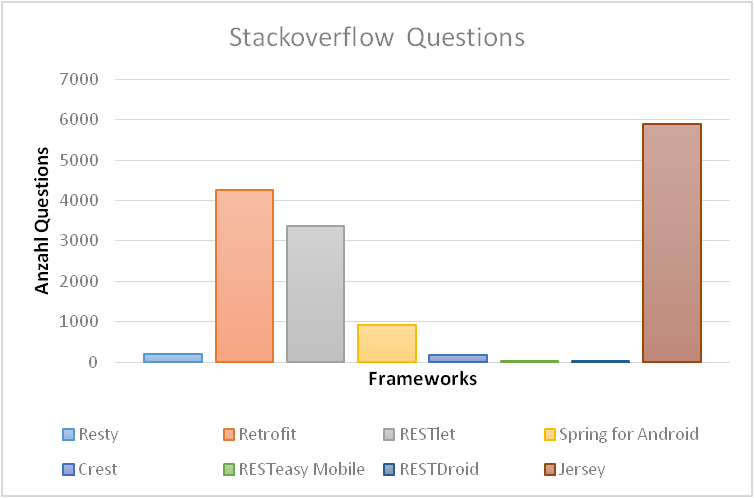
\includegraphics[width=0.65\textwidth]{figures/stackoverflow_questions.png}
	\captionof{figure}{Stackoverflow Questions, abgerufen am 24.09.2015}	
	\label{figure:stackoverflowQuestions}
	\vspace{2ex}
\end{minipage}

\begin{minipage}{\textwidth} 
	\centering	
	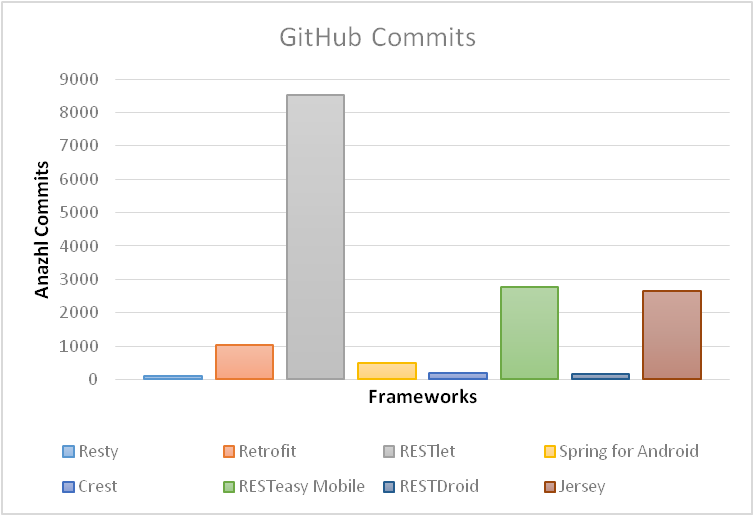
\includegraphics[width=0.65\textwidth]{figures/github_commits.png}
	\captionof{figure}{Github Commits, abgerufen am 25.09.2015}	
	\label{figure:githubCommits}
	\vspace{2ex}
\end{minipage}

\begin{minipage}{\textwidth} 
	\centering	
	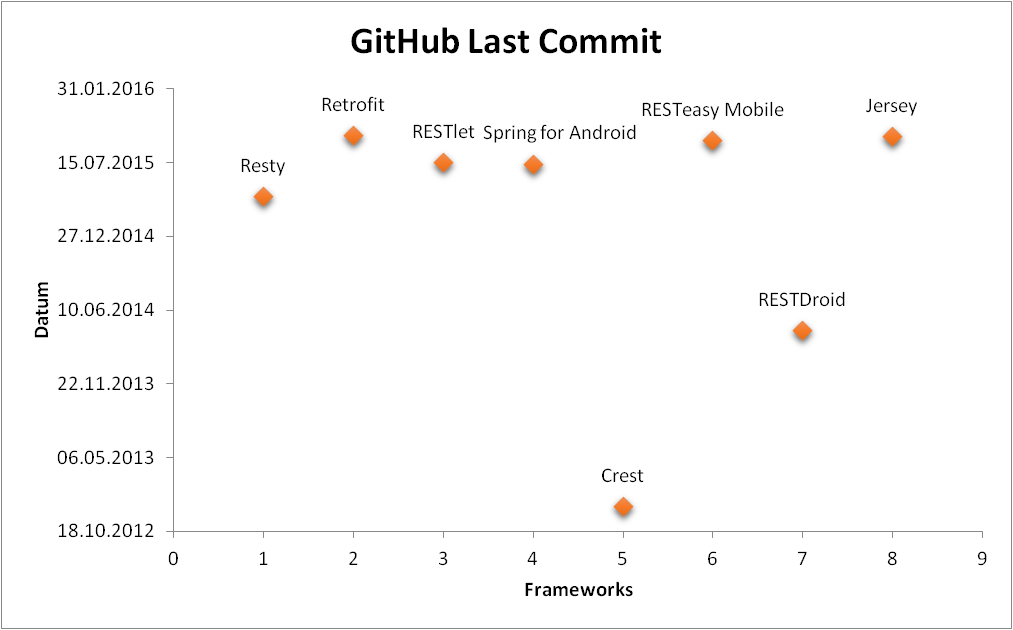
\includegraphics[width=0.65\textwidth]{figures/github_lastCommit.png}
	\captionof{figure}{GitHub Last Commit, abgerufen am 28.09.2015}	
	\label{figure:githubLastCommit}
	\vspace{5ex}
\end{minipage}

Aufgrund der Vorstudie werden folgende REST-Frameworks evaluiert und miteinander verglichen:

\begin{itemize}
	\item Retrofit 
	\item Jersey
	\item Spring for Android
\end{itemize}
%%%%%%%%%%%%%%%%%%%%%%%%%%%%%%%%%%%%%%%%%%%%%%%%%%%%%%%%%%%%%%%%%%%%%%%%
\chapter{Rest}
\label{sec:rest}
%%%%%%%%%%%%%%%%%%%%%%%%%%%%%%%%%%%%%%%%%%%%%%%%%%%%%%%%%%%%%%%%%%%%%%%%
Der Architekturstil \acrlong{REST}, kurz \acrshort{REST} wurde erstmals im Jahr 2000 in der Dissertation von Roy Fielding vorgestellt. REST beschreibt dabei ein Konzept, dass die Prinzipien des World Wide Web zusammenfasst. Roy Fielding abstrahierte sich dabei von konkreten Architekturen wie dem \acrfull{HTTP} oder \acrfull{URI}. Er legte nur Kernprinzipien fest, die mit unterschiedlichen Protokollen umgesetzt werden können. Zum Beispiel wie Ressourcen im WEB identifiziert oder adressiert werden \cite{fielding:restDis}. \\
\\
Es werden dabei folgende 5 Kernprinzipien unterschieden \cite{restHttp:book}: 
\begin{enumerate}
	\item \textbf{Ressourcen mit eindeutiger Identifikation}\\
	Durch einen global definierten Namensraum wird sichergestellt, dass Ressourcen weltweit eindeutig identifiziert werden. Im Web heißt dieses Konzept für die Vergabe von IDs, \textit{Uniform Resource Identifier} oder kurz URI. 
	
	\item \textbf{Hypermedia}\\
	Mithilfe dieses Konzeptes ist es mögliche andere Ressourcen zu referenzieren, um beispielsweise an zusätzliche Informationen zu gelangen. Ein weiterer wichtiger Aspekt ist die Möglichkeit die Applikation durch Links zu steuern. Ein Server kann dem Client über Hypermedia-Elemente mitteilen, welche Aktion er als Nächstes auszuführen hat - indem der Client einen Link \textit{folgt}. Dies wird auch oft als das \acrfull{HATEOAS}-Konzept bezeichnet. 
	
	\item \textbf{Standardmethoden}\\
	Jede Ressource unterstützt den gleichen Satz an Methoden, mit dem diese verarbeitet werden können. Bei HTTP zählen dazu folgende:
	\begin{itemize}
		\item GET, für die Dartstellung von Ressourcen
		\item POST, für das Erstellen einer Ressource
		\item PUT, für das Aktualisieren einer Ressource
		\item DELETE, für das Löschen einer Ressource
		\item HEAD, um Methadaten einer Ressource Abzurufen
		\item OPTION, um die unterstützten Methoden einer Ressource zu erhalten
	\end{itemize}
	
	\item \textbf{Unterschiedliche Repräsentationen}\\
	HTTP verfolgte einen Ansatz zur Trennung der Verantwortlichkeiten, für Daten und Operationen. Ein Client der ein bestimmtes Dateiformat verarbeiten kann, ist in der Lage jede Ressource mit diesem Format zu verarbeiten, da die Operationen dafür dieselben sind. 
	
	\item \textbf{Statuslose Kommunikation}\\
	Serverseitig wir der Zustand des Clients nicht gespeichert. Der aktuelle Zustand muss vollständig auf Seiten des Clients abgespeichert werden und bei Reqeuests müssen die nötigen Informationen an den Server übermittelt werden.
	
\end{enumerate}


%%%%%%%%%%%%%%%%%%%%%%%%%%%%%%%%%%%%%%%%%%%%%%%%%%%%%%%%%%%%%%%%%%%%%%%%
\chapter{Vergleich}
\label{sec:comparison}
%%%%%%%%%%%%%%%%%%%%%%%%%%%%%%%%%%%%%%%%%%%%%%%%%%%%%%%%%%%%%%%%%%%%%%%%
Es folgt nun eine Gegenüberstellung der einzelnen Frameworks, anhand der in Kapitel \ref{sec:methodik} definierten Kriterien. Als erster wird ein genereller Überblick über die einzelnen Fakten zu den Frameworks gegeben und deren Unterschiede beschrieben. Danach wird genauer auf relevanten Kriterien für das Revex Projekt eingegangen und ein persönliches Fazit zu den Frameworks gegeben.

\section{Gegenüberstellung der Frameworks}

{\large \textbf{Entwicklungskultur rund um die Frameworks}}\\\\
Alle Frameworks werden unter einer Open Source Lizenz zur Verfügung gestellt. Einige Lizenzen beinhalten aber ein Copyleft, was verlangt, dass die entwickelte Software ebenfalls wieder unter der gleichen Lizenz als \acrfull{OSS} zur Verfügung gestellt wird. Die wichtigste Copyleft-Lizenz ist die \acrfull{GPL}. Die GPL bestimmt, dass Software, welche eine Framework unter dieser Lizenz nutzt, wiederum nur unter GPL vertrieben werden darf. Die Apache License ist eine Lizenz ohne Copyleft, es ist daher zulässig Frameworks mit dieser Lizenz in proprietärer Software zu verwenden. Die \acrfull{CDDL} beinhaltet ein abgeschwächtes Copyleft, lizenzierter Code kann in einem anderen Framework verwendet werden, solange dieser Code nicht auf Dateiebene gemischt wird. Die CDDL verbietet nicht, entwickelte Software unter einer anderen Lizenz zu veröffentlichen. Für die reinen Nutzer von OSS, welche die Frameworks weder weiterentwickeln noch vertreiben wollen, spielen die Unterschiede der verschiedenen OSS-Lizenzen kaum eine Rolle. Will ein Entwickler jedoch seine Arbeitsergebnisse nicht als OSS veröffentlichen, darf er für seine Arbeiten keine OSS Frameworks verwenden, welche mit einem strengen Copyleft lizenziert sind \cite{openSource}. Die Lizenzen der einzelnen Frameworks könnten aus der Tabelle \ref{tableVergleich} entnommen werden.
\\\\
OSS wird durch Communities entwickelt, weiterentwickelt und gewartet. Dabei übernimmt die Community zahlreiche Aufgaben, die bei Closed Software vom Hersteller oder Anbieter wahrgenommen werden. In der Regel gibt es zu jeder OSS genau eine Community. User der Software können dabei registriertes Mitglied der Community sein und aktiv am Projekt als Entwickler oder Tester mitarbeiten. Die Qualität einer Software hängt dabei maßgeblich von der Aktivität und der Struktur der Community ab. Sind zahlreiche aktive Mitglieder mit unterschiedlichen Rollen am Projekt beteiligt, ist dies eine Grundlage für eine gute Qualität der Software \cite{openSource:community}. Alle untersuchten Frameworks weisen eine aktive und starke Community auf.
\\\\
Um die Anwendung neuer Frameworks zu lernen, lesen 78 Prozent der Entwickler die Dokumentation, 55 Prozent verwenden Codebeispiele und 29 Prozent fragen Kollegen \cite{robillard:apis}. Dadurch ist es besonders wichtig auf eine aktuelle Dokumentation des Source-Codes Zugriff zu haben. Wird nur eine veraltete Dokumentation zur Verfügung gestellt, kann es passieren das die entwickelte Software Sicherheitslücken hat oder mehr Zeit für eine korrekte Implementierung benötigt wird \cite{lethbridge:documentation}. Für alle Frameworks ist eine Dokumentation vorhanden. Die Dokumentation von Retrofit deckt dabei aber nur die grundlegend Funktionsweise ab und ist im Vergleich zu den anderen schwächer. Ein Problem hierbei ist, dass gerade ein großes Update des Frameworks durchgeführt wurde und die vorhandene Dokumentation dadurch teilweise veraltet ist. Es konnten auch Codebeispiele für alle Frameworks gefunden werden, diese sind gut erklärt und ermöglichen es eine lauffähige Anwendung zu implementieren. Problematisch war es allerdings die gefunden Jersey Codebeispiele unter Android zu starten, da keines dieser speziell für Android entwickelt wurde. Es musste zuerst ein Workaround (siehe Kapitel \ref{workaroundAndroid}) durchgeführt werden, um die Beispiele auf einem Android Gerät starten zu können.
\\\\
{\large \textbf{Implementierung der REST-Frameworks}}\\\\
Einer der relevantesten Aspekte für den Evaluierungsprozess ist die Implementierung und Verwendungsweise der Frameworks. Bis auf Jersey sind alle Frameworks leicht einzubinden und zu benützen. Für Jersey muss zuerst ein Workaround durchgeführt werden, damit dieses Framework überhaupt unter Android genutzt werden kann. Die genaue Verwendungsweise der Frameworks wird in Kapitel \ref{chapter:frameworks} beschrieben.
\\\\
Es werden von allen Frameworks die gängigsten HTTP-Methoden unterstützt. Retrofit unterstützt dabei als einziges nicht die HTTP-Methode OPTIONS. Es ist auch möglich mit allen Frameworks den HTTP-Header zu erweitern bzw. zu verändern. Des weiteren ist es auch möglich alle möglichen Medientypen zu unterstützten, wenn ein Konverter dafür implementiert und beim Framework registriert wird. Endpoint URLs zum Server können dynamisch während der Laufzeit bei allen Frameworks verändert werden. 
\\\\
Wenn zeitraubende Aktionen ausgeführt werden sollen, wie z.B. das Herunterladen einer großen Dateien aus dem Internet, langweilen sich User oft. Denn diese müssen dann warten bis der Request vollständig abgearbeitet wurde und können währenddessen nicht weiterarbeiten. Dies kann aber verhindert werden, indem zeitraubende Aktion im Hintergrund ausgeführt werden - in Form von asynchronen Requests \cite{louis:android}. Mithilfe aller Frameworks können asynchrone Requests modelliert werden. 
\\\\
Das HATEOAS Konzept wird von Jersey und Spring for Android unterstützt. Jedoch muss bei Spring for Android eine eigene Bibliothek \textquotedblleft Spring HATEOAS\textquotedblright eingebunden werden, damit eine Linkverfolgung möglich ist. Wenn das HATEOAS Konzept mit AndroidAnnotations verwendet werden soll, muss ebenfalls \textquotedblleft Spring HATEOAS\textquotedblright eingebunden werden und die Verwendung ist nur ohne Annotations möglich. Man greift dabei auf die Basis REST Implementierung zurück, welche Spring for Android ist. Retrofit unterstützt das HATEOAS Konzept nicht.
\\\\
Das registrieren von Error Handlern ist bei allen Frameworks möglich, dadurch können aussagekräftige Fehlermeldungen für den User erzeugt werden. Designrichtlinien für mögliche Geräte geben an, dass es sinnvoll ist Rückmeldungen für Aktion des Systems zu geben, wie beispielsweise eine Fehlermeldung, wenn der Server nicht erreichbar ist. Eine solche Rückmeldung sollte für den Benutzer verständlich sein. Zum Beispiel sind die Fehlermeldungen \textquotedblleft HTTP404 ERROR\textquotedblright und \textquotedblleft Diese Seite konnte nicht gefunden werden \textquotedblright äquivalent, die zweite Fehlermeldung ist aber für einen größteil der User verständlicher \cite{gong2004guidelines}.
\\\\
{\large \textbf{Performance}}\\\\
Mobile Geräte haben längst Einzug in das Alltagsleben erhalten, viele Nutzer erweitern die Funktionalität der Geräte mit zahlreichen Anwendungen. Jede installierte App auf einen mobilen Endgerät hat Einfluss auf den Energieverbrauch. Je mehr Anwendungen auf eine Endgerät installiert sind und je öfter diese genutzt werden, desto höher ist der Energieverbrauch und die Betriebszeit sinkt dadurch massiv \cite{Wil2012}. Daher ist bei der Entwicklung darauf zu achten, das der Energieverbrauch so gering wie möglich gehalten wird. Auswirkungen auf den Energieverbrauch eines Smartphones haben sowohl der Bildschirm, die \acrfull{CPU}, die Kommunikation über das Mobilfunknetz, als auch das WLAN-Modul. Werden die einzelnen Komponenten so wenig wie möglich beansprucht, ist der Energieverbrauch der Anwendung gering \cite{vetter}. 
\\\\
Umso länger und mehr Daten bei einem Request über das Mobilfunknetz oder das WLAN-Modul übertragen werden, desto mehr Energie wird verbraucht. Es sollte daher darauf geachtet werden, dass die Requestdauer möglichst gering ist und nicht unnötige Daten übertragen werden. Des weiteren ist die Rechenleistung von Smartphones  wesentlich geringer als jene von Notebooks, um die Betriebszeit zu erhöhen. Daher ist bei der Entwicklung auch darauf zu achten, dass die CPU Beanspruchung der Apps gering gehalten wird, damit das System performant weiterarbeiten kann \cite{mittal:energy}. Außerdem sollte die benötigte CPU Leistung aus einem weiteren Grund möglichst gering sein, den die Hardware variiert von Smartphone zu Smartphone. Ist die benötigte CPU Leistung gering, ist es möglich die App auf nahezu allen mobilen Geräten zu installieren und zu starten \cite{joorabchi:challenges}. 
\\\\
Für den Performance Vergleich wurden daher sowohl die CPU-Auslastung, als auch die Dauer für GET- und POST Requests (Dauer der Netzwerkkommunikation) der einzelnen Frameworks gegenübergestellt. Um Vergleichswerte zu ermitteln, wurden jede App einzeln in einem Emulator gestartet und die gleich Abfolge an Funktionsaufrufen durchgeführt. 
\\\\
Die Zeitdauer der GET-Requests bei der Abbildung \ref{getRequests} setzt sich aus 11 einzeln abgesetzte GET-Requests zusammen. Diese Requests werden benötigt, um die Details zu einem bestimmten Kraftwerke anzuzeigen. Es werden in der Praxis oft mehrere GET-Request hintereinander abgesetzt, daher wurde die Dauer ermittelt um alle Details zu einem Kraftwerk abzurufen. Es konnte dabei festgestellt werden, dass Retrofit die Daten am schnellsten überträgt, dicht gefolgt von AndroidAnnotations und Jersey am langsamsten ist.

\begin{figure} [ht]
	\centering
	\subfloat[GET Request Retrofit]{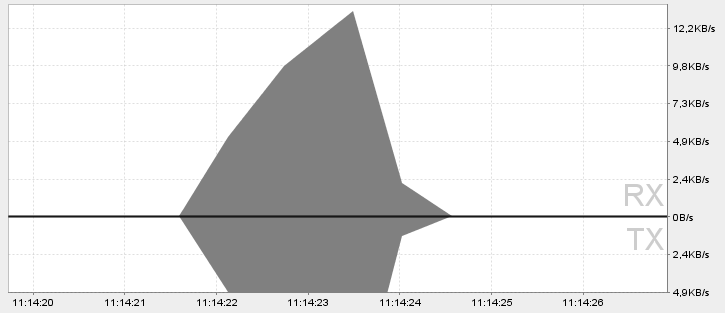
\includegraphics[width=0.45\textwidth]{figures/get_retrofit.png}} \qquad
	\subfloat[GET Request Jersey]{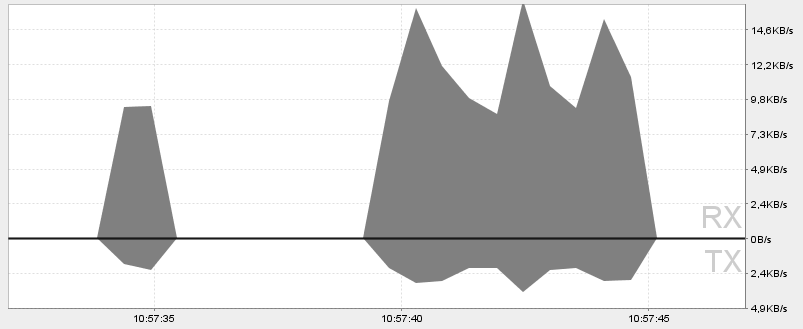
\includegraphics[width=0.45\textwidth]{figures/get_jersey.png}} \qquad
	\subfloat[GET Request Spring for Android]{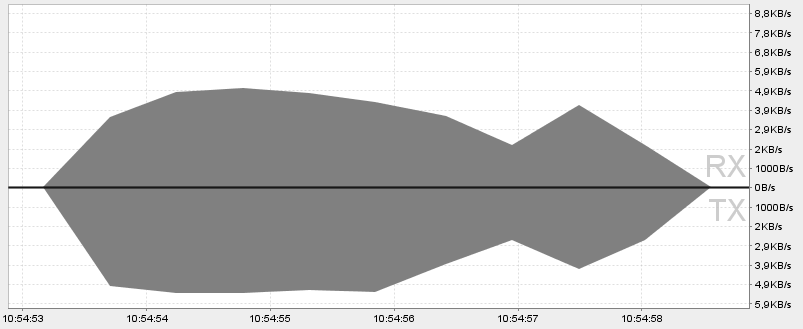
\includegraphics[width=0.45\textwidth]{figures/get_spring.png}} \qquad
	\subfloat[GET Request AndroidAnnotations]{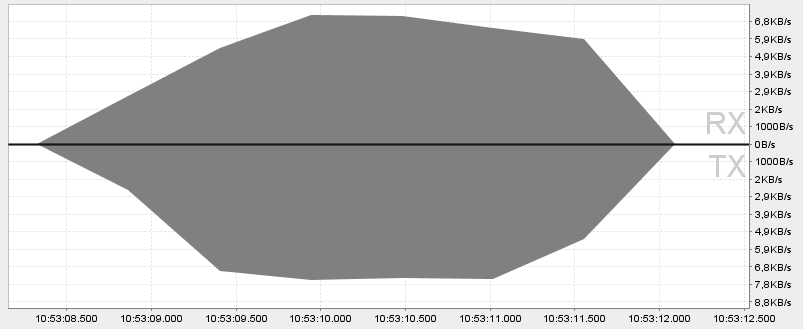
\includegraphics[width=0.45\textwidth]{figures/get_aa.png}}
	\caption{Zeitmessung der GET Requests} 
	\label{getRequests}
\end{figure} 

\newpage
Die Messung der Zeitdauer für einen POST Request ist aus der Abbildung \ref{postRequests} zu entnehmen. Dabei wurde die Zeit gemessen bis neu eingegeben Daten, um ein Kraftwerk anzulegen erfolgreich zum Server übermittelt wurden. Es konnte dabei festgestellt werden, dass alle Frameworks circa gleich lange benötigen, um die Daten zu übertragen. Spring for Android ist dabei minimal langsamer als die anderen, dies ist aber zu vernachlässigen, da diese Verzögerung keine Auswirkung auf die Usability für einen User hat \cite{meyer:performance}.

\begin{figure} [ht]
	\centering
	\subfloat[POST Request Retrofit]{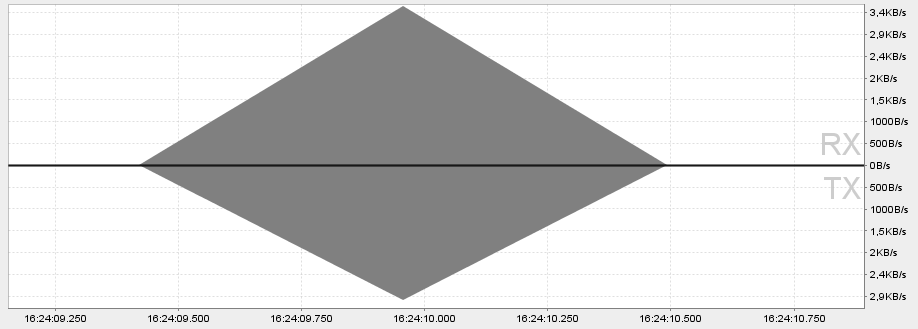
\includegraphics[width=0.45\textwidth]{figures/post_retrofit.png}} \qquad
	\subfloat[POST Request Jersey]{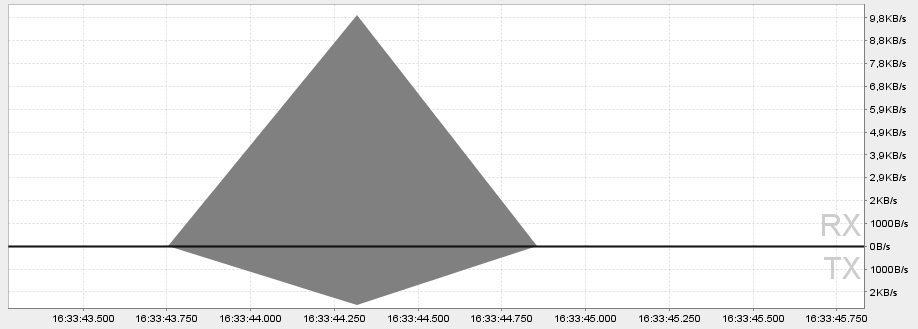
\includegraphics[width=0.45\textwidth]{figures/post_jersey.png}} \qquad
	\subfloat[POST Request Spring for Android]{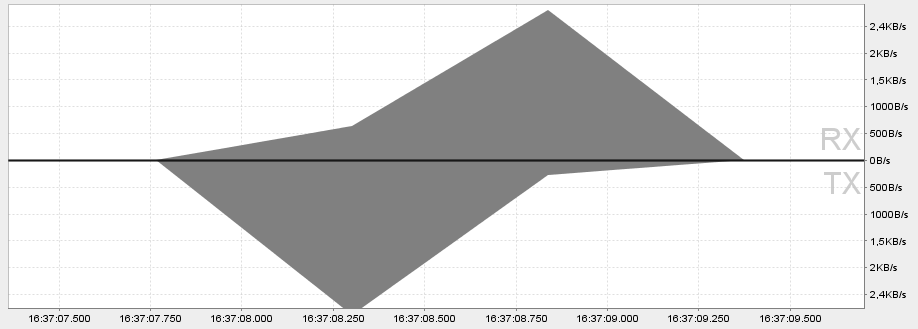
\includegraphics[width=0.45\textwidth]{figures/post_spring.png}} \qquad
	\subfloat[POST Request AndroidAnnotations]{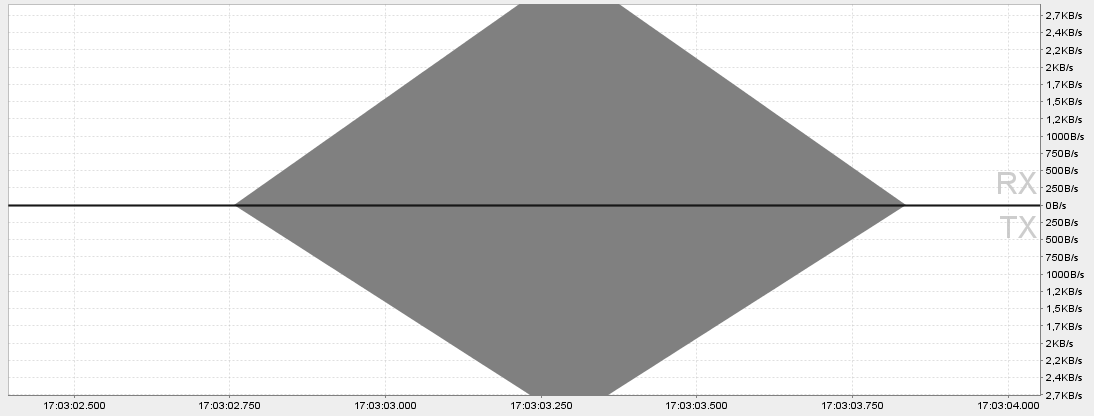
\includegraphics[width=0.45\textwidth]{figures/post_aa.png}}
	\caption{Zeitmessung der POST Requests} 
	\label{postRequests}
\end{figure} 

In der Abbildung \ref{cpuAuslastung} wird die CPU Auslastung der einzelnen Frameworks gegenübergestellt. Aus dieses Abbildung kann entnommen werden, das AndroidAnnotations die CPU am geringsten in Anspruch nimmt und Jersey am stärksten. Bei der Benutzung der Apps ist auch festzustellen, dass AndroidAnnotations und Retrofit am schnellsten arbeiten und eine flüssige Bedienung der Anwendung möglich ist. Jersey ist des öfteren langsam und hat kleine Ruckler währende der Bedienung.  

\begin{figure} [ht]
	\centering
	\subfloat[CPU Auslastung Retrofit]{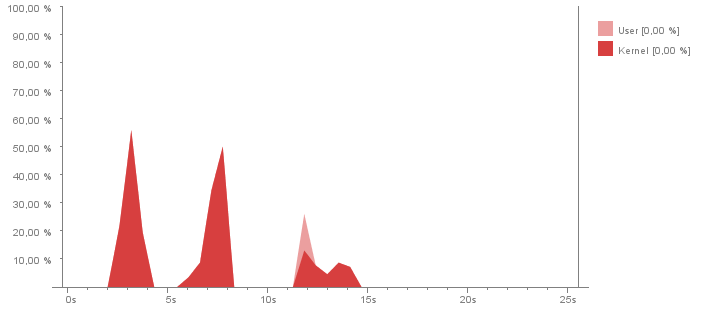
\includegraphics[width=0.45\textwidth]{figures/cpu_retrofit.png}} \qquad
	\subfloat[CPU Auslastung Jersey]{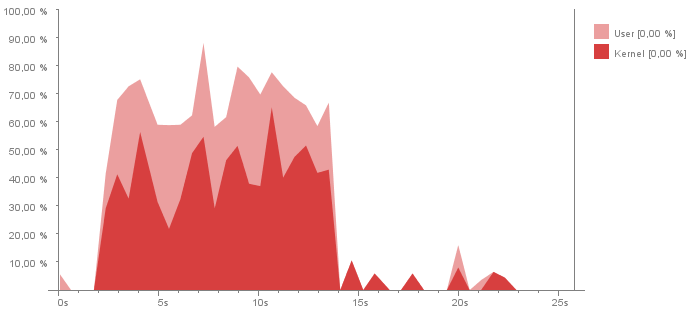
\includegraphics[width=0.45\textwidth]{figures/cpu_jersey.png}} \qquad
	\subfloat[CPU Auslastung Spring for Android]{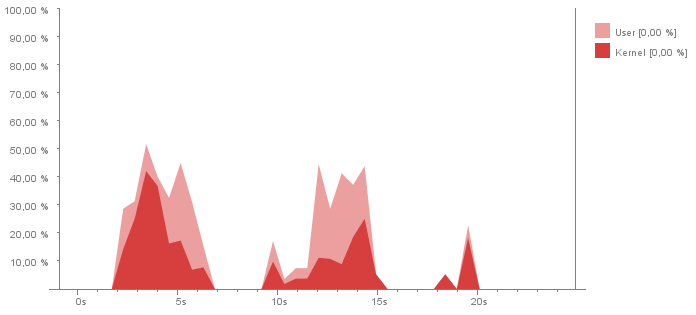
\includegraphics[width=0.45\textwidth]{figures/cpu_spring.png}} \qquad
	\subfloat[CPU Auslastung Request AndroidAnnotations]{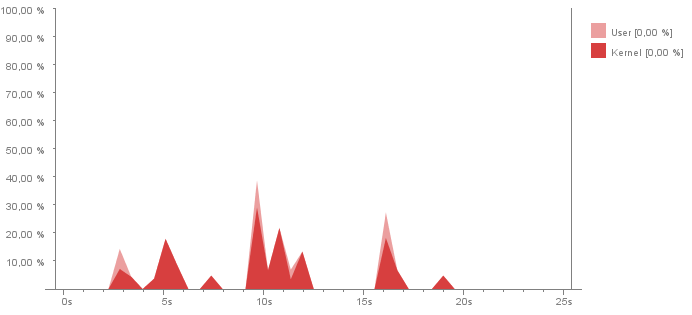
\includegraphics[width=0.45\textwidth]{figures/cpu_aa.png}}
	\caption{CPU Auslastung} 
	\label{cpuAuslastung}
\end{figure} 

{\large \textbf{Speicherplatz}}\\\\
Eine der größten Herausforderungen beim Implementieren von Apps ist der Hardwareunterschied der mobilen Geräte. Die Hardwarekomponenten unterscheiden sich nicht nur in der Displaygröße oder CPU Leistung, sondern auch im Speicherbereich \cite{joorabchi:challenges}. Sei es nun der zur Verfügung gestellte \acrfull{RAM} oder interne Speicher, welcher gelegentlich durch Speicherkarten erweitert werden kann. Je mehr und je größere Apps installiert werden, desto mehr leidet die Performance – insbesondere auf älteren oder Hardware schwachen Geräten. Auch spielt die Installationszeit eine wichtige Rolle. User wollen Apps so schnell wie möglich nutzen, längere Installationszeiten sorgen schneller dafür, dass die Installation abgebrochen wird \cite{schaefers:apk}. Bei der Gegenüberstellung der APK Größe und der maximalen RAM Beanspruchung schnitt AndroidAnnotations am besten ab, Jersey am schlechtesten (siehe Tabelle \ref{tableVergleich}). 

\begin{figure} [ht]
	\centering
	\subfloat[benötigter RAM Retrofit]{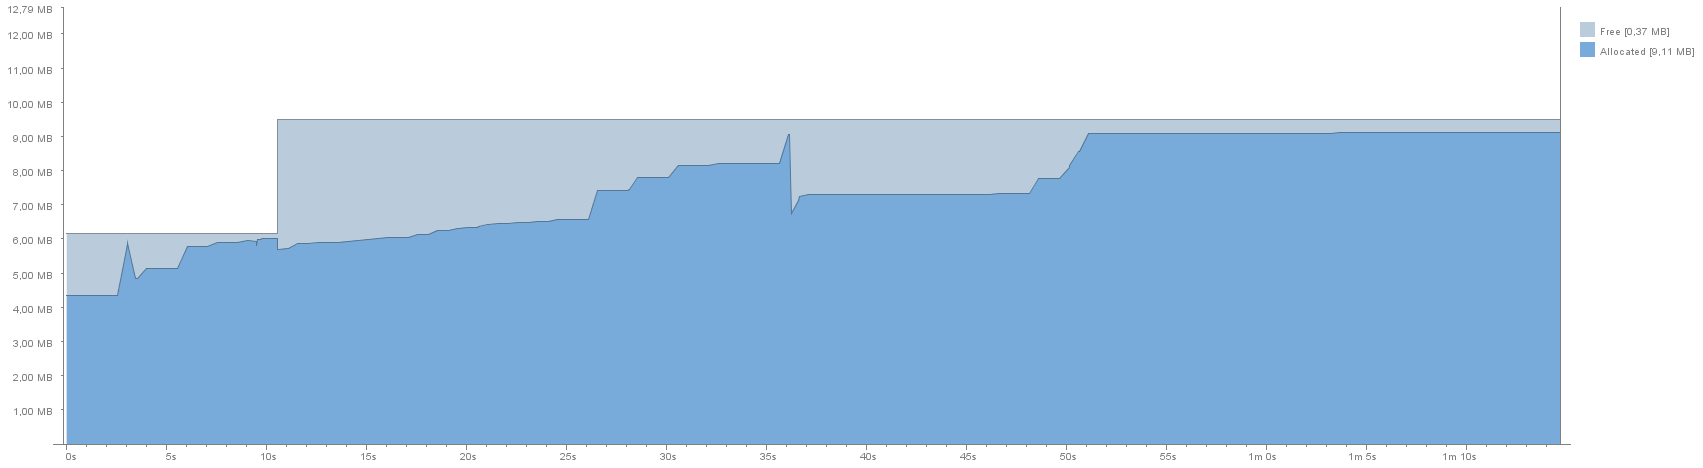
\includegraphics[width=0.48\textwidth]{figures/ram_retrofit.png}} \qquad
	\subfloat[benötigter RAM Jersey]{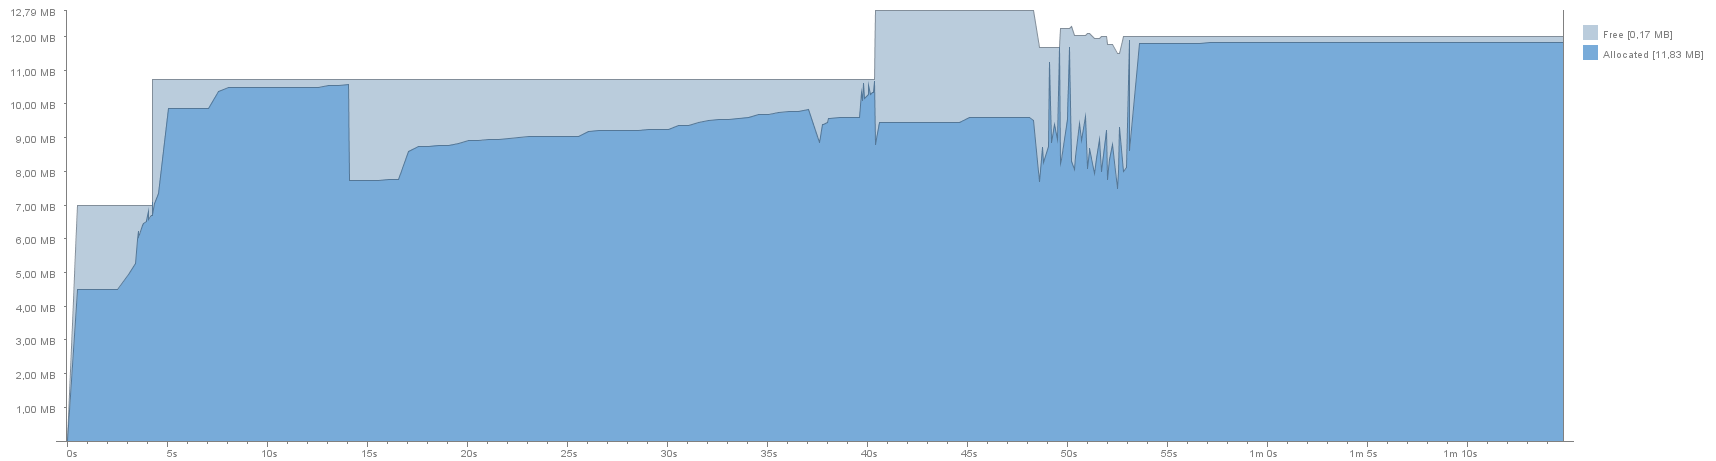
\includegraphics[width=0.45\textwidth]{figures/ram_jersey.png}} \qquad
	\subfloat[benötigter RAM Spring for Android]{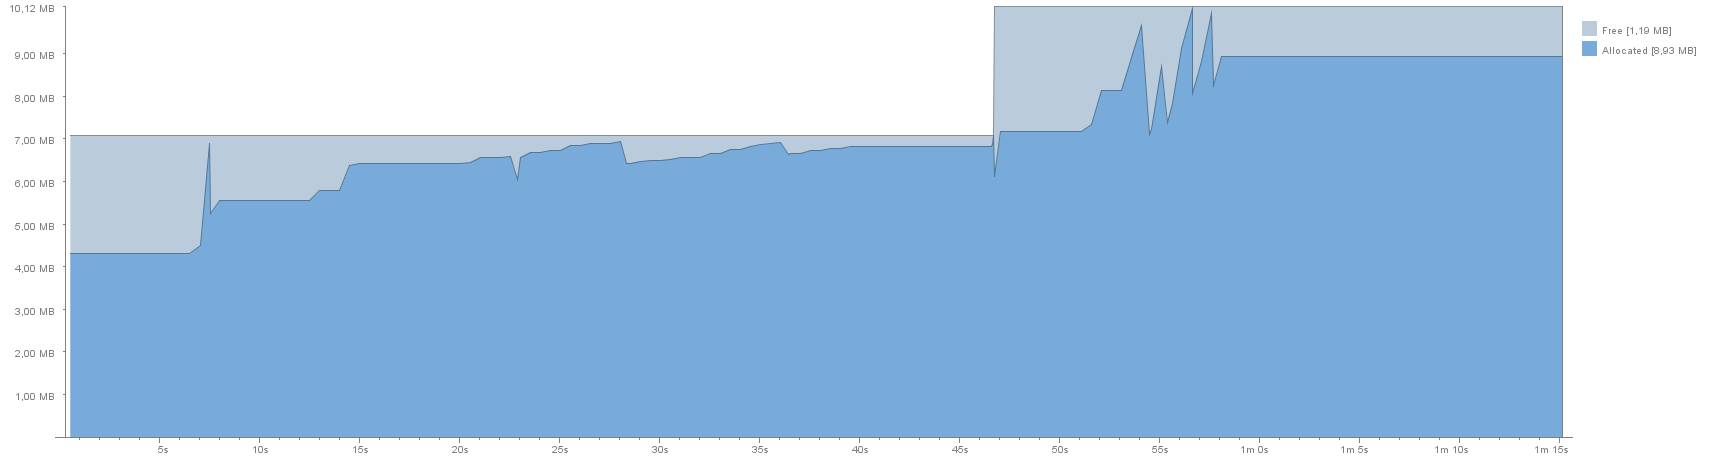
\includegraphics[width=0.45\textwidth]{figures/ram_spring.png}} \qquad
	\subfloat[benötigter RAM Request AndroidAnnotations]{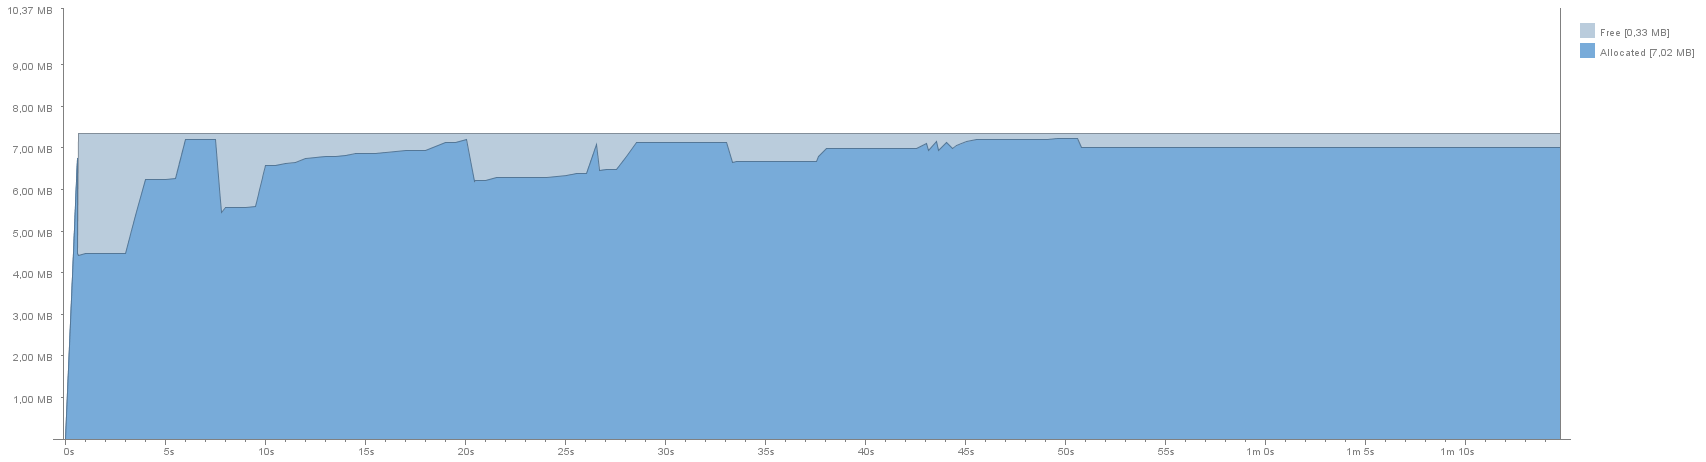
\includegraphics[width=0.45\textwidth]{figures/ram_aa.png}}
	\caption{benötigter RAM} 
	\label{ramB}
\end{figure} 

{\large \textbf{Erweiterte Technische Fähigkeiten der Frameworks}}\\\\
Sicherheit ist ein wesentliches Thema in der Informatik und auch für mobile Geräte. Denn die Apps sind nicht nur auf Informationen des Smartphones beschränkt, sondern haben auch Zugriff auf das Internet. OAuth ist ein Webstandard für den beschränkten Zugriff von Benutzer-Ressourcen auf Servern \cite{shehab:secure}. Dieser Standard wir von allen Frameworks unterstützt und ermöglicht einen sicheren und beschränkten Zugriff auf Ressourcen. 
\\\\
Alle evaluierten Frameworks unterstützten keine weiteren Übertragungsprotokolle außer HTTP. Die ACID-Eigenschaften werden auch von keinem der Frameworks implementiert. Soll aber ein Transaktionsmanagement clientseitig unterstützten werden, muss eine eigene Implementierung geschrieben werden. Dabei muss besonders darauf geachtet werden, dass alle Daten, die während einer Transaktion verwendet werden, gesperrt sind und sich nicht ändern dürfen so lange bis die Transaktion Commited wird oder ein Rollback durchgeführt wird \cite{braun:Transaktionen}.
\\\\
Jersey hat eine serverseitige Referenzimplementierung. Für Spring for Android existiert ebenfalls eine Referenzimplementierung aus der Spring Familie. AndroidAnnoations hat keine direkt Referenzimplementierung, aber man kann auch auf jene der Spring Familie zurückgreifen - den die REST Implementierung von AndroidAnnoations basiert auf Spring for Android. Retrofit hat keine serverseitige Referenzimplementierung.
\\\\
AndroidAnnotations stellt als einziges Framework zusätzliche Dienste bereit, welche die Implementierung einer Android App erleichtern. Diese zusätzlichen Dienste sind unter anderem Dependency Injection oder Event Binding, siehe Kapitel \ref{androidannoations}.
  
\begin{landscape}
% m{3.5cm}|m{4.5cm}|m{4.5cm}|m{4.5cm}|m{4.5cm}
\renewcommand{\arraystretch}{1.3}
\begin{longtable}{m{3.5cm}|m{4.5cm}|m{4.5cm}|m{4.5cm}|m{4.5cm}}
	%	>{\centering \arraybackslash}m{3.5cm}|
	%	>{\centering \arraybackslash}m{4.5cm}|
	%	>{\centering \arraybackslash}m{4.5cm}|
	%	>{\centering \arraybackslash}m{4.5cm}|
	%	>{\centering \arraybackslash}m{4.5cm}}

      \caption{Gegenüberstellung der Frameworks} \\
	  \label{tableVergleich}	 
	  
	    & \textbf{Retrofit} & \textbf{Jersey} & \textbf{Spring for Android}  & \textbf{AndroidAnnotations}  \\  \hhline{=====}
	   \multicolumn{5}{c}{\textbf{Entwicklungskultur}} \\ \hhline{=====}
	  \textbf{Lizenz} &
	  Apache License Version 2.0 & CDDL Version 1.1 \newline GPL Version 2 & 
	  Apache License Version 2.0 & 
	  Apache License 2.0 \newline CDDL \\ \hline
	  \textbf{aktive Community} & Ja & Ja & Ja & Ja\\ \hline
	  \textbf{Dokumentation} & grundlegend & gut & gut  & gut \\ \hline 
		  \textbf{Codebeispiele} &  Ja  & nicht speziell für Android & Ja & Ja\\ \hhline{=====}
	  
	  \multicolumn{5}{c}{\textbf{Implementierung}} \\ \hhline{=====}
	  \textbf{Einbindung} & leicht & problematisch & leicht & leicht \\ \hline
	  \textbf{HTTP-Methoden} & GET, POST, PUT, DELETE, HEAD & GET, POST, PUT, DELETE, HEAD, OPTIONS  & GET, POST, PUT, DELETE, HEAD, OPTIONS & GET, POST, PUT, DELETE, HEAD, OPTIONS \\ \hline
	  \textbf{HTTP-Header} & erweiterbar & erweiterbar & erweiterbar & erweiterbar \\ \hline
	  \textbf{unterstützte\newline Medientypen} & alle möglichen, wenn Konverter für Typ vorhanden ist & alle möglichen, wenn Konverter für Typ vorhanden ist & alle möglichen, wenn Konverter für Typ vorhanden ist & alle möglichen, wenn Konverter für Typ vorhanden ist \\ \hline
	  \textbf{URL veränderbar} & Ja & Ja & Ja & Ja  \\ \hline
	  \textbf{asynchrone Requests} & Ja & Ja & Ja & Ja \\ \hline
	  \textbf{HATEOAS Konzept} & Nein & Ja & mithilfe von Spring HATEOAS & ohne Annotations und mithilfe von Spring HATEOAS \\ \hline 
	  \textbf{Error-Handling} & unterstützt & unterstützt & unterstützt & unterstützt \\ \hline
	 \newpage \hhline{=====}
	  
	  \multicolumn{5}{c}{\textbf{Performance und Speicherplatz}} \\ \hhline{=====}
	  
	  \textbf{GET Request} & \textasciitilde3s & \textasciitilde12s  & \textasciitilde5s & \textasciitilde3.5s\\ \hline
	  
	  \textbf{POST Request} & \textasciitilde1s &  \textasciitilde1s & \textasciitilde1.5s & \textasciitilde1s \\ \hline
	  
	  \textbf{CPU Auslastung} & max. \textasciitilde55\%  & max. \textasciitilde87\% & max. \textasciitilde52\% & max. \textasciitilde40\%\\ \hline
	  \textbf{belegter RAM} & max. 9.11 MB & max. 11.83 MB & max. 8.93 MB & max 7.02 MB \\ \hline
	  \textbf{APK Größe} & 1.70 MB & 2.58 MB & 1.69 MB & 1.44 MB \\ \hhline{=====}

	   \multicolumn{5}{c}{\textbf{Erweiterte Technische Fähigkeiten}} \\ \hhline{=====}
	   
	   \textbf{Sicherheit} & OAuth2, SSL via OkHttp & OAuth2, SSL & OAuth2, SSL & OAuth2, SSL \\ \hline
	   \textbf{andere Protokolle außer HTTP} &  Nein & Nein & Nein & Nein\\ \hline	   
	   \textbf{ACID-Eigenschaften} & Nein & Nein & Nein & Nein \\ \hline
	   \textbf{Server Implementierung} & Nein & Ja &  Spring Framework & Nein (eventuell Spring Framework) \\ \hline
	   \textbf{zusätzliche Dienste} & Nein & Nein & Nein & Ja \\ \hline
 
\end{longtable}
\end{landscape}

\section{Relevante Aspekte für Revex2020}
Für die Implementierung einer App sind sowohl Retrofit, Spring for Android und AndroidAnnoations geeignet. Von Jersey als REST Framework ist abzuraten, da dieses Framework nur mithilfe eines Workarounds benützt werden kann. Darüber hinaus schneidet Jersey im Performance- und Speichervergleich am schlechtesten ab. Vergleicht man nun jene anderen drei ist der Unterschied minimal. Retrofit weißt eine etwas schwächere Dokumentation auf, da gerade eine neue Version erschienen ist und die Dokumentation teilweise noch nicht an die neueste Version angepasst wurde. Spring for Android ist im Lesezugriff langsamer, was einen minimalen Nachteil darstellt - da dies das Hauptaugenmerk einer Implementierung für Revex ist. Retrofit und AndroidAnnoations haben einen leicht zu lesenden Code, da dieser Annotations basiert ist. Dadurch verringert sich der zu schreibende und wartende Code, wodurch die Entwicklung beschleunigt und die Wartbarkeit verbessert werden kann. Der größte Vorteil von AndroidAnnoations sind die zusätzlicher Dienste, welche die Implementieren einer Android App erleichtern.

\section{Persönliches Fazit zu den Frameworks}
Es folgt nun ein kurzer persönlicher Eindruck zu den Frameworks. Wo sind Probleme während der Implementierung aufgetreten und welche Aspekte besonders positiv aufgefallen sind.
\\\\
\textbf{Jersey}
\\\\
\textbf{Retrofit}
\\\\
\textbf{Spring for Android}
\\\\
\textbf{AndroidAnnotations}
\\\\

% insert bibliography and such stuff
\BackMatter
\cleardoublepage

\appendix
%%%%%%%%%%%%%%%%%%%%%%%%%%%%%%%%%%%%%%%%%%%%%%%%%%%%%%%%%%%%%%%%%%%%%%%%%
\chapter{\appendixlabel}
%%%%%%%%%%%%%%%%%%%%%%%%%%%%%%%%%%%%%%%%%%%%%%%%%%%%%%%%%%%%%%%%%%%%%%%%



\end{document}
